\section{Calorimeter cluster reconstruction}
\label{sec:clusterselection}
\subsection{Definition}
EMCal clusters are formed by a clustering algorithm that combines signals from adjacent towers. We use calorimeter clusters defined with the ``V1'' algorithm. This algorithm starts from a ``seed" cell, found from a local-maximum scan, and adds ``neighbor" cells to the cluster if they are above a given threshold. The cluster definition is exclusive, i.e. once a cell is assigned to a cluster, it is not considered for other clusters. The minimum energy for the seed and neighbor were set to 500 and 100 MeV respectively; these values are several times larger than the standard deviation of the electronic noise\footnote{Some photon analysis use a 50 MeV threshold, but 100 MeV has been found to improve cell time measurements. The 100 MeV threshold has been used for example in Ref~\cite{Acharya:2017tlv}.}.

\subsection{Corrections}
We apply several corrections at the cell level, implemented within the ``EMCal Correction Framework,"\footnote{\url{http://alidoc.cern.ch/AliPhysics/master/_r_e_a_d_m_eemc_corrections.html} } before the clustering algorithm is run over the data and simulations. The following corrections are applied: 
\begin{itemize}
\item ``\textsc{CellEnergy}"\\
This performs an energy calibration of cells, with coefficients obtained with $\pi^{0}\to\gamma\gamma$ mass measurements.
\item ``\textsc{CellBadChannel}''\\
This removes cells that declared hot or dead for a given run period. 
\item ``\textsc{CellTimeCalib}"\\
This correction applies constant offsets, which are arbitrary, to the cell time measurements to minimize the spread among cells. 
\item ``\textsc{CellEmulateCrosstalk}''. \\
This correction, described in detail in Ref~\cite{CrossTalk}, modifies the simulated cell energies to emulate the cell cross-talk that has been observed in data. This is applied to all the simulations described in Table~\ref{tab:MCsamples}. 
\end{itemize}

\subsection{Selection}
The following selection is applied on the resulting clusters\footnote{This event selection also closely follows previous and concurrent isolated-photon spectra analyses in pp and \pPb~ data.}:

\begin{itemize}
\item Cluster $\pt$ cut:  $12< \pt < 40$ \GeVc.
\item Cluster pseudorapidity: $|\eta| <0.67$\\
The cluster pseudorapidity is corrected for the position of the primary interaction vertex. 
\item Number of cells cut: $N_{\mathrm{cell}}\geq2$\\
This requirement removes clusters that are likely dominated by noise. 
\item Exoticity cut: $E_{\mathrm{cross}}/E_{\mathrm{cluster}}$ $> 5\%$\\
We remove ``exotic'' or ``spiky'' clusters likely coming from slow neutrons or highly-ionizing particles hitting the avalanche photo-diode of a cell by a requirement on the ratio of the summed energy around the leading cell to the total cluster energy.
\item Cluster time cut:  $|t|<20$ [ns]\\
We require a cluster time measurement of $|t|<$ 20 ns to remove out-of-bunch pileup. 
\item Number of local maxima cut: $N_{LM}<$ 3\\
This cuts suppresses background and improves the MC simulation description of the background~\cite{Acharya:2019jkx}.  
\item Distance seed-cell to bad-channel$\geq 1$ cells.
\end{itemize}

Figures~\ref{ClusterCutFlow_pPb} and~\ref{ClusterCutFlow_pp} show the distribution of the variables used in the cluster selection and the effect of sequential selection (``cut flow") for the \pPb~and pp data respectively. Table~\ref{tab:photonCutFlow} shows a summary of the effect of sequential selection on the number of selected clusters in both pp and \pPb~data. 

\begin{figure}[h]
\center
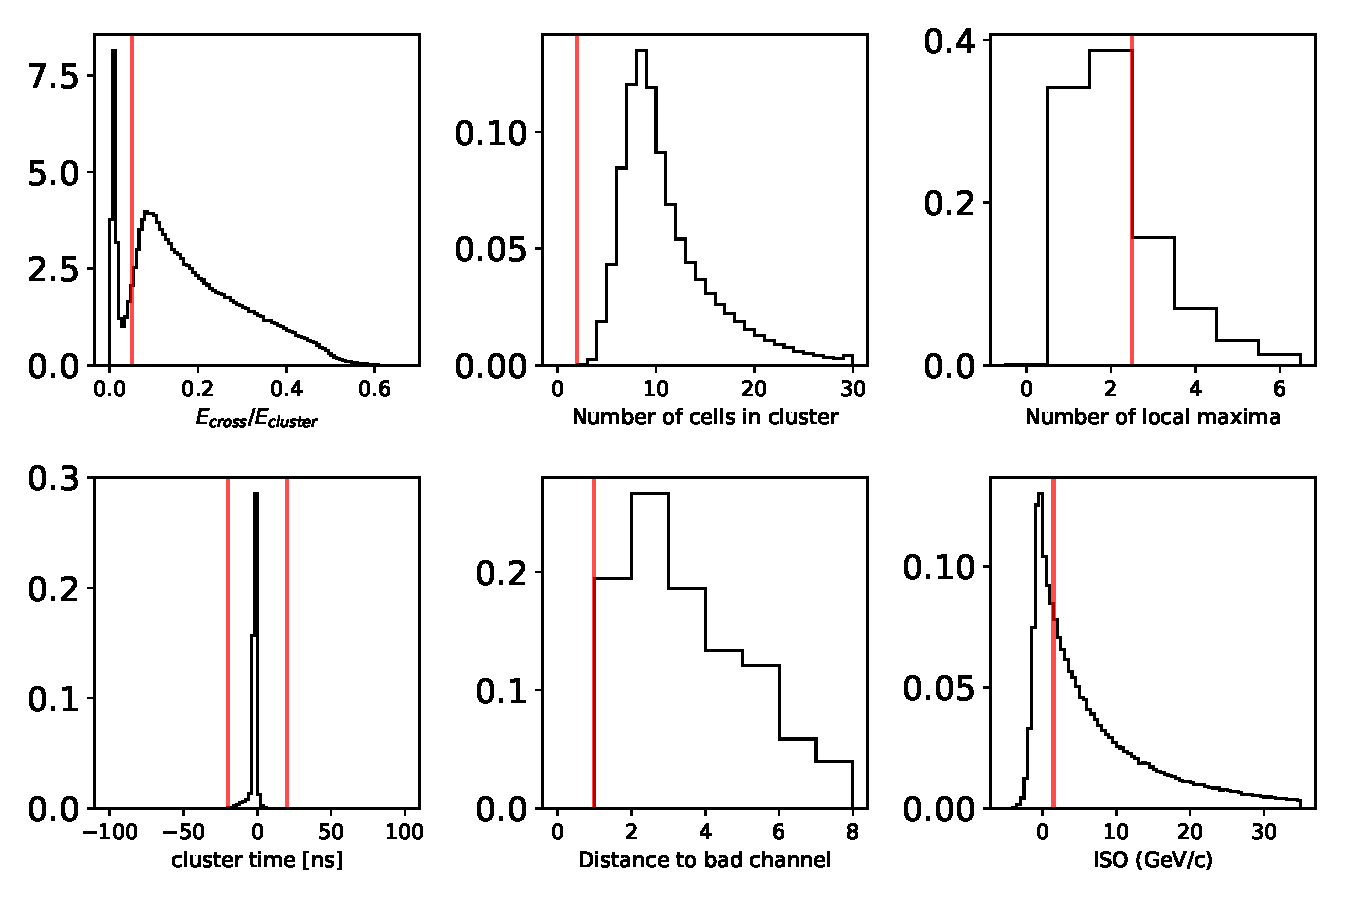
\includegraphics[width=0.95\textwidth]{EventAndClusterSelection/ClusterCutFlow_dataset_Skimmed_13def}
\caption{Distribution of variables used in the cluster selection of \pPb~data. The red vertical lines represent the cuts used. The cluster cuts get applied sequentially, i.e. the clusters cut with a given variable do not appear in the next.}
\label{ClusterCutFlow_pPb}
\end{figure}


\begin{figure}[h]
\center
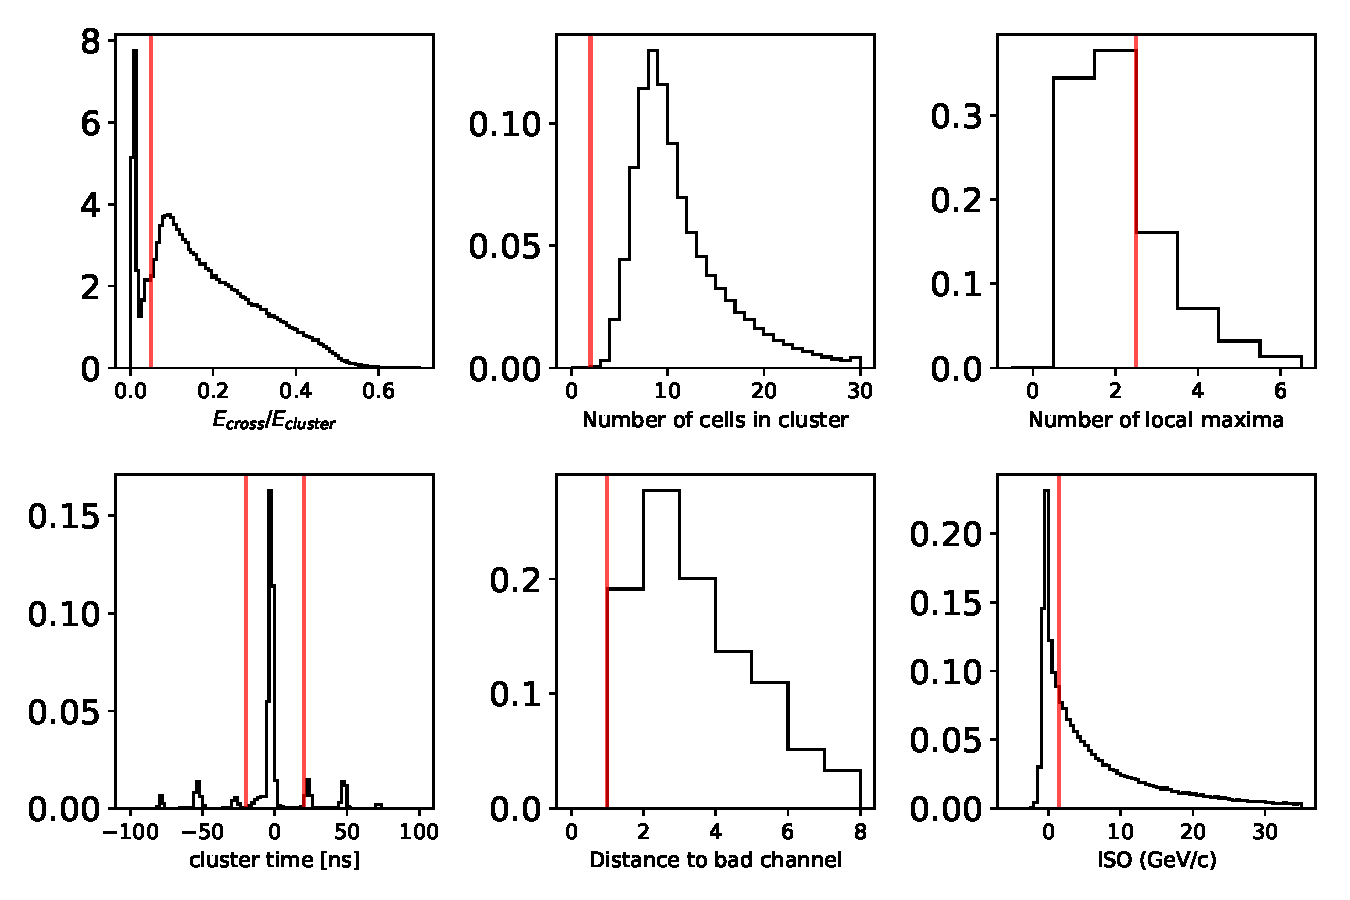
\includegraphics[width=.95\textwidth]{EventAndClusterSelection/ClusterCutFlow_dataset_Skimmed_17q}
\caption{Distribution of variables used in the cluster selection in pp data. The red vertical lines represent the cuts used. The cluster cuts get applied sequentially, i.e. the clusters cut with a given variable do not appear in the next.}
\label{ClusterCutFlow_pp}
\end{figure}


\begin{table}[h]
   \centering
   \caption{Number of clusters, with  $12<\pt<40$ \GeVc, that pass our selection in 2013 \pPb~and 2017 pp data.}
   \label{tab:photonCutFlow}
   \begin{tabular*}{1.0\columnwidth}{@{\extracolsep{\fill}}lcc@{}}
    \hline
       Selection  &  \pPb~ data & pp data  \\
       \hline
       $|\eta| < 0.67$& 714834 & 385220  \\
      $E_{\mathrm{cross}}/E_{\mathrm{cluster}}$ $> 5\%$ & 613560 & 323750   \\
       $N_{\mathrm{cell}}$ $\geq 2$   &613560& 323750       \\
              $N_{LM}<$ 3 & 443102&231490 \\
       $|t|<20$ [ns] &441639 & 171470  \\ 
       Distance-to-bad channel $\geq 1$ &441639  &171470  \\ 
       $\iso<$  1.5~\GeVc & 137895  & 58638 \\ 
       0.1 $< \sigma^2_{\textrm{long}}<$  0.3  & 40027 & 16628  \\ 
       \hline
	   %Total clusters passing $\gammaiso$ selection & 38415  & 16,586 %\\ 
       %\hline
   \end{tabular*}
\end{table}

%Table~\ref{tab:mcCutFlow} shows a summary of the effect of sequential selection on the number of selected clusters in various simulated samples. This shows that in simulation, a much larger fraction of the total number of clusters passes the exoticity cut than in data. This is attributed to the fact that the simulation does not describe the albedo neutrons or energetic particles hitting the APD of the cell readout. The dijet simulation describes the cut flow relatively well, including the number of local maxima and the isolation criteria that is described in detail in Section~\ref{sec:isolation}.

%\begin{table}[h]
%\vspace*{0cm}
%   \centering
%   \caption{Fraction of clusters, with  $12~\GeVc < \pt < 30$ \GeVc, that pass our selection in simulated data. The percentage refer to the sequential application of each cut.}
%   \label{tab:mcCutFlow}
%   \hspace*
%   {-2.8cm}\begin{tabular}{@{\extracolsep{\fill}}lcccc@{}}
%    \hline
%    &  Pythia $\gamma$-jet + UE & Pythia dijet-jet + UE &  Pythia $\gamma$-jet & Pythia dijet-jet\\
%    &   17g6a1 & 17g6a3 & 18b10a(b)\_calo & 18g7a(b)\_calo\\ \hline
%    $|\eta| < 0.67$&  100$\%$ & 100$\%$ & 100$\%$ & 100$\%$\\
%    $E_{\mathrm{cross}}/E_{\mathrm{cluster}}$ $> 5\%$ & 97$\%$ & 97.8$\%$ & 97.5$\%$ & 96.3$\%$\\
%    $N_{\mathrm{cell}}$ $> 2$    &  99.9$\%$ & 100$\%$ & 100$\%$    & 100$\%$ \\
%
%	$|t|<20$ [ns] & 100$\%$ & 100$\%$ & -$\%$ & -$\%$ \\ 
%	Number of local maxima $< 3$ & 98.4$\%$ & 88.9$\%$ & 87.8$\%$ & 64.2$\%$\\ \hline
%    Fraction that pass all cuts above& 95.4$\%$ & 86.9$\%$ & 85.6$\%$ & 61.8$\%$ \\ \hline 
%	Fraction that pass all cuts above that also pass ISO cut& 91.1$\%$ & 40.3$\%$ & 86.8$\%$ & 14.6$\%$ \\ 		\hline
%    Fraction that pass all cuts & 86.9$\%$ & 35.0$\%$ & 74.3$\%$ & 9.0$\%$ \\ \hline 
%   \end{tabular}
%\end{table}
%Tables fractions need to be remade with latest MC samples. 


%\subsection{Selection Efficiency}
%The efficiency for the combined effect of all the selection cuts we used, with the exception of the isolation selection that is discussed in more detail in Section~\ref{sec:isolation}, is shown in Figure~\ref{fig:ClusterSelectionEfficiency}. The various efficiencies for the different cases are as follow: \pPb~: 0.91, pp-EMCal+DCal: 0.90, pp-EMCal: 0.91, pp-DCal: 0.79. These efficiencies were obtained by applying a constant fit to each case. 
%\begin{figure}[h]
%\center
%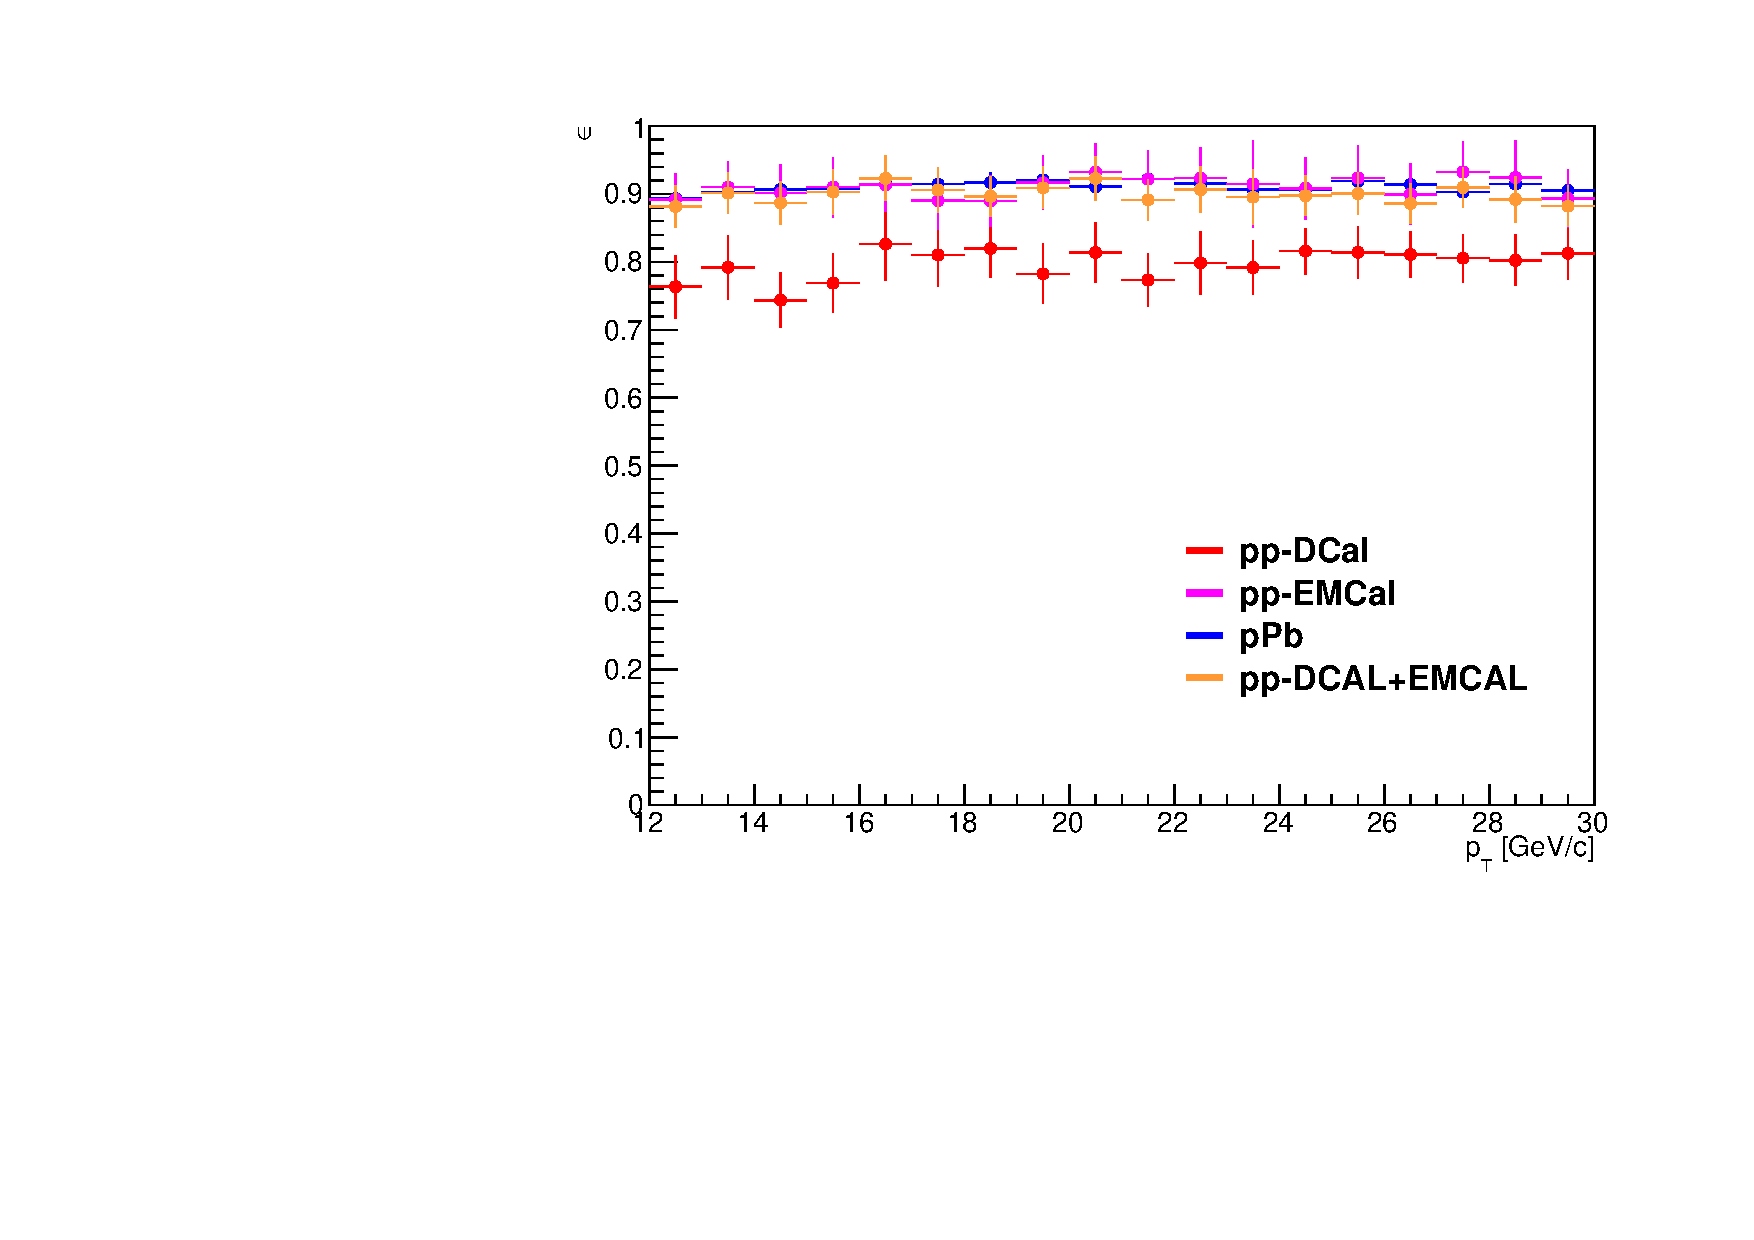
\includegraphics[width=0.5\textwidth]{EfficiencyAppendix/EfficiencyComparison_photons.pdf}
%\caption{Cluster selection efficiency for pp and \pPb~ data taking periods. The error bar represents statistical uncertainty only.}
%\label{fig:ClusterSelectionEfficiency}
%\end{figure}

%We do not use this efficiency in our analyzes because we report quantities normalized to the number of photons. However, in principle the efficiency could enter as a second-order bias if it varied rapidly with $\pt$~and we reported measurements in wide $\pt$~intervals. We note from Figure~\ref{fig:ClusterSelectionEfficiency} that this is not the case, i.e. the efficiency is almost constant for the $\pt$~range analyzed here.

%The number of cells in the cluster peaks at around 8 and has a tail to larger values, but a spike at low values; the requirement of $N_{\mathrm{cell}}>2$ removes about 10$\%$ of the clusters. The $E_{\mathrm{cross}}/E_{\mathrm{cluster}}$ variable peaks at around 0.1 and has a smooth tail to larger values that reach up to around 0.6. A peak at small values is attributed to ``exotic'' clusters that are the product of albedo neutrons or minimum-ionizing particles hitting the APD of the cell, which producing large signal in a single cell but not in their neighbors~\cite{ExoticClusters}. The exoticity cut, $E_{\mathrm{cross}}/E_{\mathrm{cluster}} >$ 0.03 rejects about 6\% of all clusters. The time cut rejects less than 1$\%$ of the clusters in \pPb~, but about a quarter in the pp dataset. Then, we reject events with more than 2 local minimum to reduce background from meson decays and hadrons, rejecting about 20\% of the remaining clusters. 
%Finally, we apply an isolation cut (described in Section~\ref{sec:isolation}) to reduce background from multi-jet events; this keeps about a third of all the clusters. 

